\scanpage{4}
\mspage{2}
\margin{\figure{\begin{tikzpicture}\draw (0,0)--(.6,-.65);\end{tikzpicture}}}

$\ell-8$\quad pourquoi\quad \uline{donc}\qquad ?

\rule{\linewidth}{0.3pt}

p3\quad $\ell-8,-9$\qquad $B$ ?

\rule{\linewidth}{0.3pt}

p4.\quad 1.3.1.\quad As tu vérifié si l'accouplement d'\unsure{A. M.} coïncide avec le tien ?

$\ell\,4$.\quad \uline{formellement} non ramifié ?

$\ell\,7$.\quad \uline{séparablement} clos ?

$\ell\,14-20$.\quad Est-ce utile à dire, en l'absence de référence à ce que ce peut vouloir dire ?

$\ell-5$\quad Qu'il soit\qquad et\qquad \unsure{signifierait}\qquad plutôt ?

\rule{\linewidth}{0.3pt}

pg5\quad $\ell-2$\quad français :\quad les classes $\unsure{w|\omega}$\qquad \uline{en}\qquad relatifs.

\rule{\linewidth}{0.3pt}

pg6\quad $\ell\,4$\quad français.\quad dire\quad un Module inversible simple\qquad ?

\deleted{\illegible{5}}

\figure{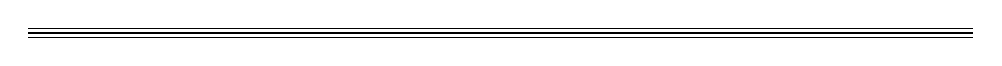
\begin{tikzpicture}\draw (0,0)--(12,0);\draw (0,-0.06)--(12,-0.06);\draw (0,-0.12)--(12,-0.12);\end{tikzpicture}}

\figure{
\begin{tikzpicture}[baseline=(t.base)]\node (t) {2};\draw (0,0) circle (0.27);\draw (0.01,0.01) ellipse (0.31 and 0.29);\end{tikzpicture}}

pg7\quad français \uline{$\ell-9$}\quad
\figure{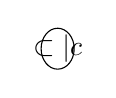
\begin{tikzpicture}[baseline=(t.base)]\node[inner sep=2pt] (t) {$\unsure{\subset|c}$};\draw (0,0) ellipse (0.21 and 0.26);\end{tikzpicture}}
$L_0$\quad donc
\figure{
\begin{tikzpicture}[baseline=(t.base)]\node[inner sep=2pt] (t) {c'};\draw (0,0) ellipse (0.23 and 0.26);\end{tikzpicture}}
est

\deleted{$\ell\unsure{-8}$\quad \unsure{si}\quad \illegible{1}\quad \unsure{que}}
\quad $\ell-7$\quad
\figure{
\begin{tikzpicture}[baseline=(t.base)]\node[inner sep=2pt] (t) {que};\draw (0,0) ellipse (0.36 and 0.24);\end{tikzpicture}}
(le $2^{\mathrm{e}}$)

\rule{\linewidth}{0.3pt}

pg8\quad français\quad $\ell\,4$\quad par exemple\quad à\inserted{\figure{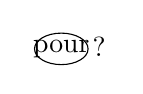
\begin{tikzpicture}[baseline=(t.base)]\node[inner sep=2pt] (t) {pour};\draw (0,0) ellipse (0.34 and 0.20);\node at (0.48,0.03) {?};\end{tikzpicture}}}\quad $\ldots$

$\ell-7$\quad \uline{le} terme

\rule{\linewidth}{0.3pt}

pg14.\quad L'argument est un peu immoral; si $X$ et $Y$ sont extensions d'une VA par un tore et si $\varphi:X\longrightarrow Y$ est donné, alors $\varphi$ est strictement compatible à la filtration par \unsure{le|les} poids et $\varphi$ est une isogénie si et seulement si $T_\ell(\varphi)$ en est une.

\rule{\linewidth}{0.3pt}

\figure{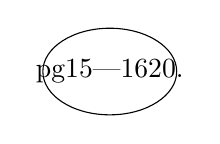
\begin{tikzpicture}[baseline=(t.base)]\node[inner sep=3pt] (t) {pg\deleted{\unsure{15|16}}20.};\draw (0,0) ellipse (0.85 and 0.55);\end{tikzpicture}}
Rmq 2.6 a)\quad $S$ est-il un trait dans cette remarque ; sait-on assez sur le passage à la limite et Néron ?

\margin{3}
